\chapter{Other Plots}

\section{Signal Fits in \texorpdfstring{$m_{KK}$}{mKK}}
\label{sec:mKK_plots}

\begin{figure}[H]
	\centering
	\captionsetup{width=0.8\linewidth}
	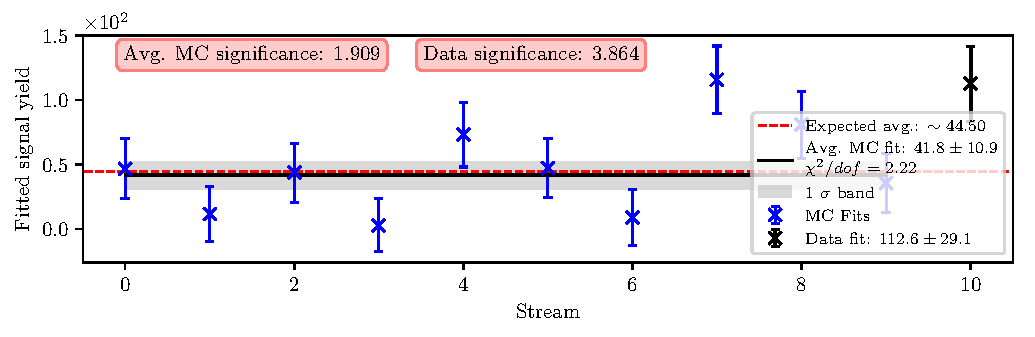
\includegraphics[width=\linewidth]{fig/sig_mKK_1}
	\caption{Signal fit result for the $1^{\mathrm{st}}$ $m_{KK}$ window for MC and data in the range $0.980<m_{KK}<1.232$.}
\end{figure}

\begin{figure}[H]
	\centering
	\captionsetup{width=0.8\linewidth}
	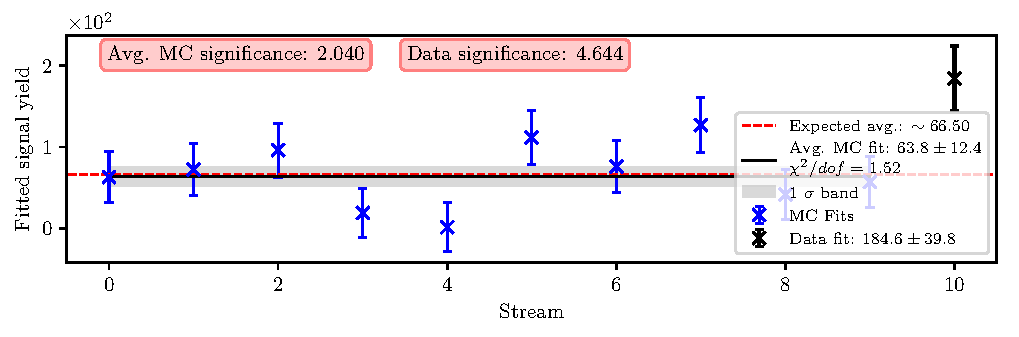
\includegraphics[width=\linewidth]{fig/sig_mKK_2}
	\caption{Signal fit result for the $2^{\mathrm{nd}}$ $m_{KK}$ window for MC and data in the range $1.232<m_{KK}<1.483$.}
\end{figure}

\begin{figure}[H]
	\centering
	\captionsetup{width=0.8\linewidth}
	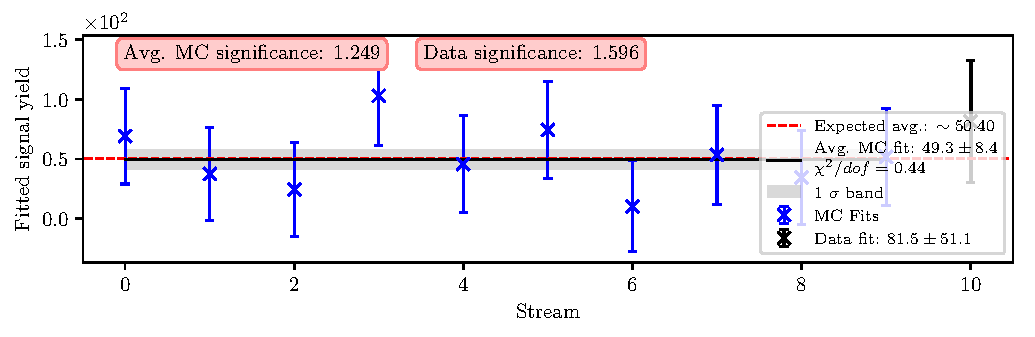
\includegraphics[width=\linewidth]{fig/sig_mKK_3}
	\caption{Signal fit result for the $3^{\mathrm{rd}}$ $m_{KK}$ window for MC and data in the range $1.483<m_{KK}<1.735$.}
\end{figure}

\begin{figure}[H]
	\centering
	\captionsetup{width=0.8\linewidth}
	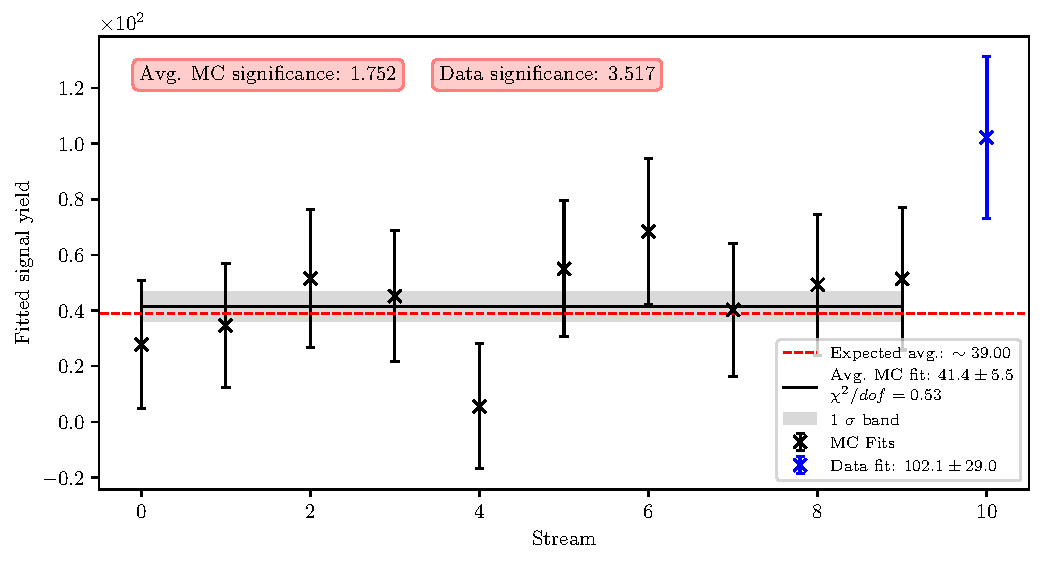
\includegraphics[width=\linewidth]{fig/sig_mKK_4}
	\caption{Signal fit result for the $4^{\mathrm{th}}$ $m_{KK}$ window for MC and data in the range $1.735<m_{KK}<1.987$.}
\end{figure}

\begin{figure}[H]
	\centering
	\captionsetup{width=0.8\linewidth}
	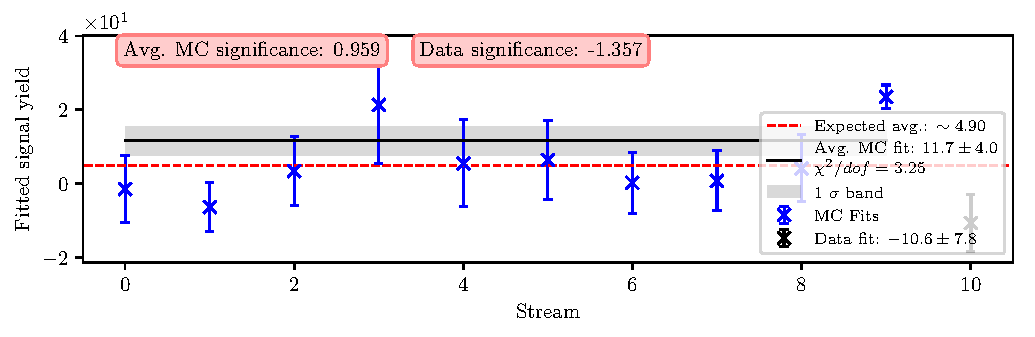
\includegraphics[width=\linewidth]{fig/sig_mKK_5}
	\caption{Signal fit result for the $5^{\mathrm{th}}$ $m_{KK}$ window for MC and data in the range $1.987<m_{KK}<2.238$.}
\end{figure}

\begin{figure}[H]
	\centering
	\captionsetup{width=0.8\linewidth}
	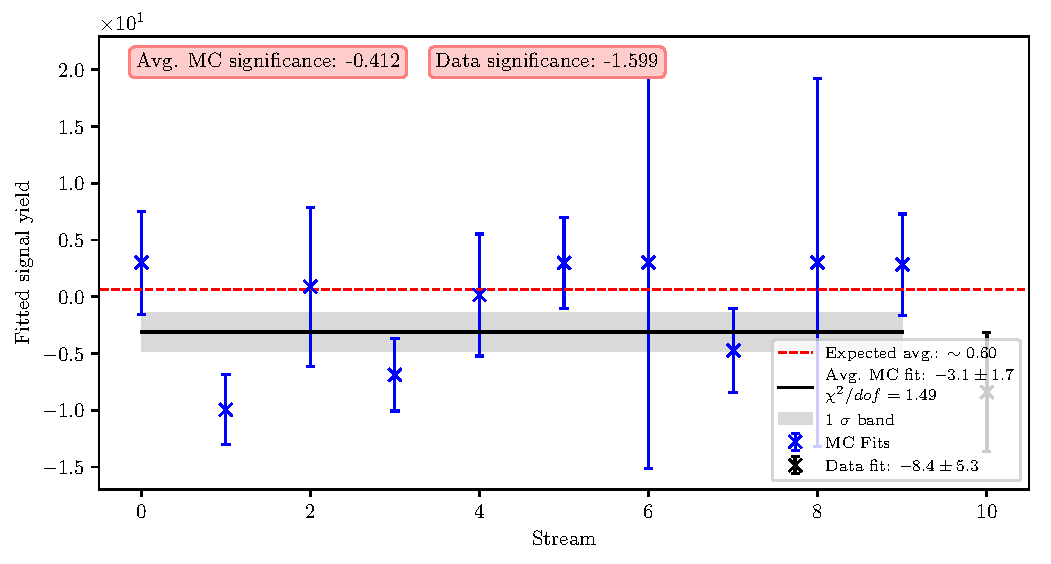
\includegraphics[width=\linewidth]{fig/sig_mKK_6}
	\caption{Signal fit result for the $6^{\mathrm{th}}$ $m_{KK}$ window for MC and data in the range $2.238<m_{KK}<2.490$.}
\end{figure}

\begin{figure}[H]
	\centering
	\captionsetup{width=0.8\linewidth}
	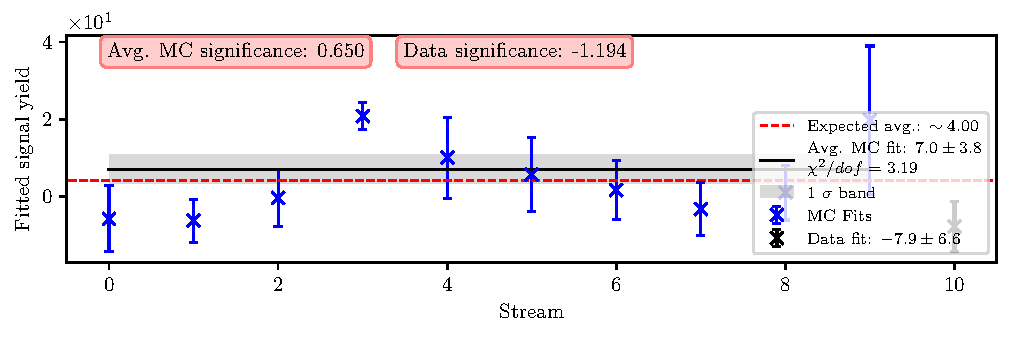
\includegraphics[width=\linewidth]{fig/sig_mKK_7}
	\caption{Signal fit result for the $7^{\mathrm{th}}$ $m_{KK}$ window for MC and data in the range $2.490<m_{KK}<2.742$.}
\end{figure}

\begin{figure}[H]
	\centering
	\captionsetup{width=0.8\linewidth}
	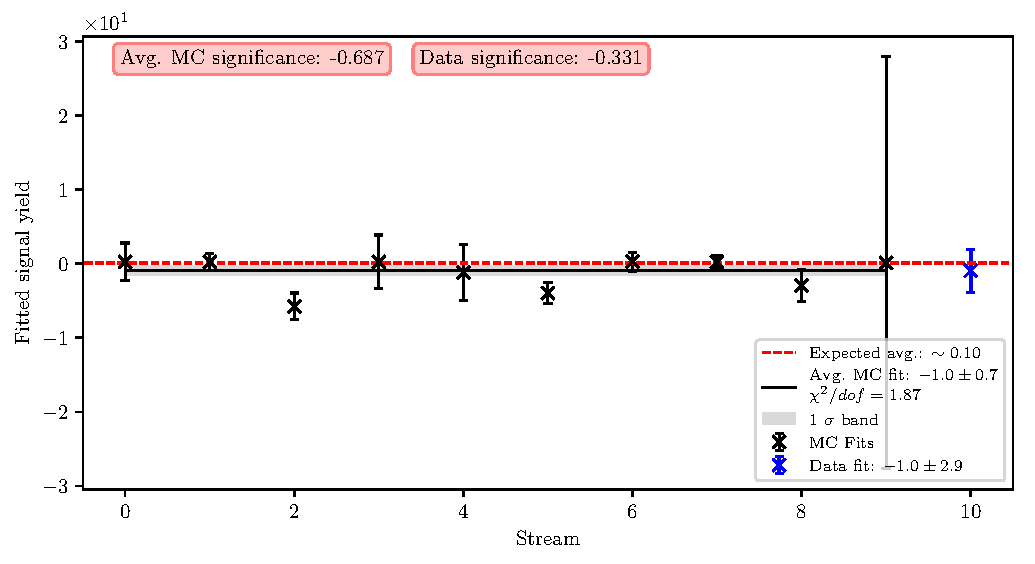
\includegraphics[width=\linewidth]{fig/sig_mKK_8}
	\caption{Signal fit result for the $8^{\mathrm{th}}$ $m_{KK}$ window for MC and data in the range $2.742<m_{KK}<2.993$.}
\end{figure}

\begin{figure}[H]
	\centering
	\captionsetup{width=0.8\linewidth}
	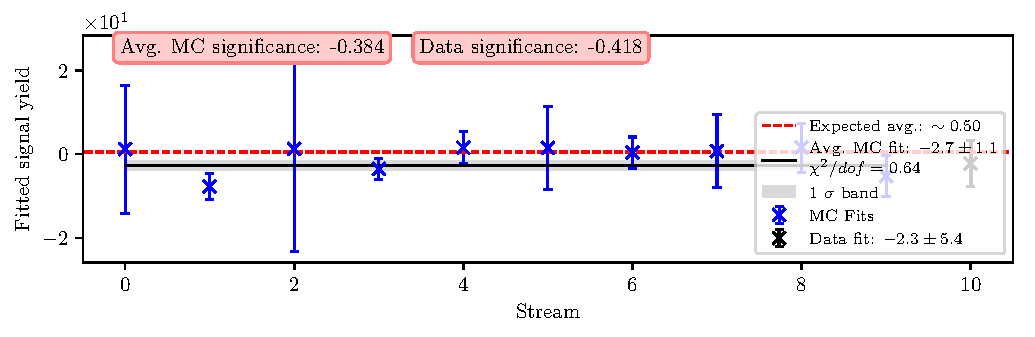
\includegraphics[width=\linewidth]{fig/sig_mKK_9}
	\caption{Signal fit result for the $9^{\mathrm{th}}$ $m_{KK}$ window for MC and data in the range $2.993<m_{KK}<3.245$.}
\end{figure}

\begin{figure}[H]
	\centering
	\captionsetup{width=0.8\linewidth}
	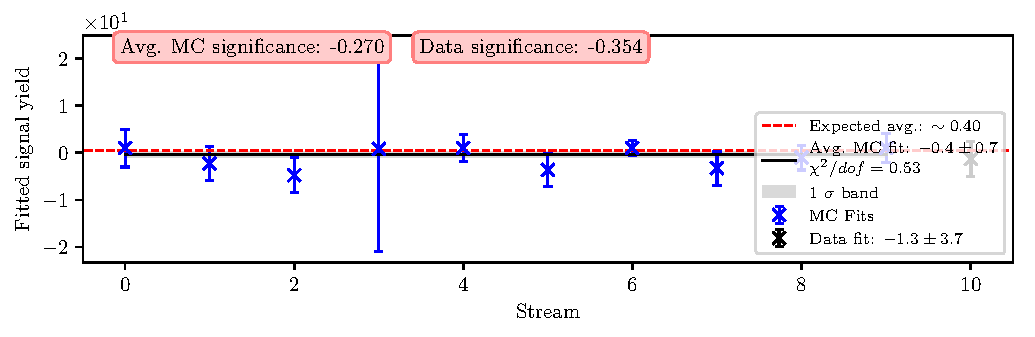
\includegraphics[width=\linewidth]{fig/sig_mKK_10}
	\caption{Signal fit result for the $10^{\mathrm{th}}$ $m_{KK}$ window for MC and data in the range $3.245<m_{KK}<3.497$.}
\end{figure}

\begin{figure}[H]
	\centering
	\captionsetup{width=0.8\linewidth}
	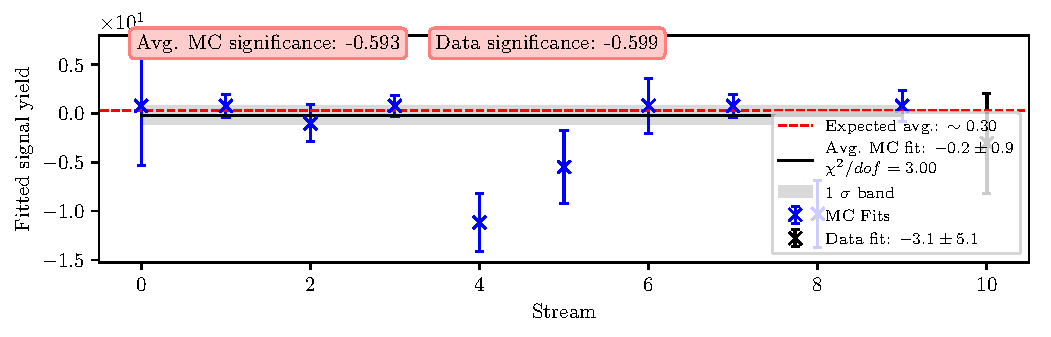
\includegraphics[width=\linewidth]{fig/sig_mKK_11}
	\caption{Signal fit result for the $11^{\mathrm{th}}$ $m_{KK}$ window for MC and data in the range $3.497<m_{KK}<3.748$.}
\end{figure}

\begin{figure}[H]
	\centering
	\captionsetup{width=0.8\linewidth}
	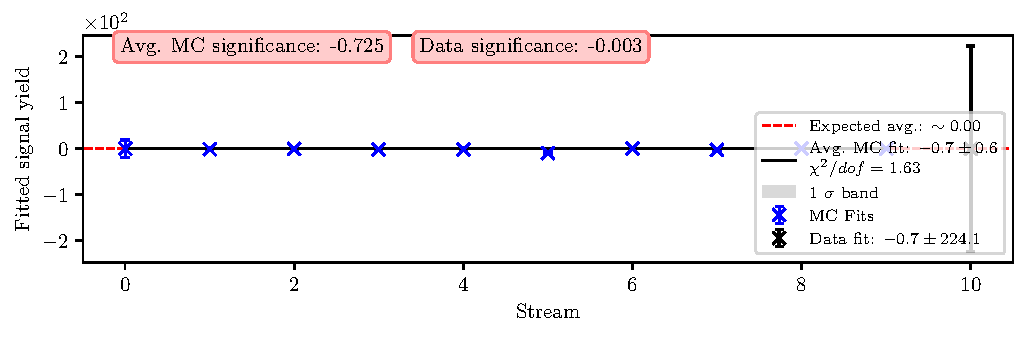
\includegraphics[width=\linewidth]{fig/sig_mKK_12}
	\caption{Signal fit result for the $12^{\mathrm{th}}$ $m_{KK}$ window for MC and data in the range $3.748<m_{KK}<4.000$.}
\end{figure}


\section{Signal Fits in \texorpdfstring{$q^2$}{q2}}
\label{sec:q2_plots}

\begin{figure}[H]
	\centering
	\captionsetup{width=0.8\linewidth}
	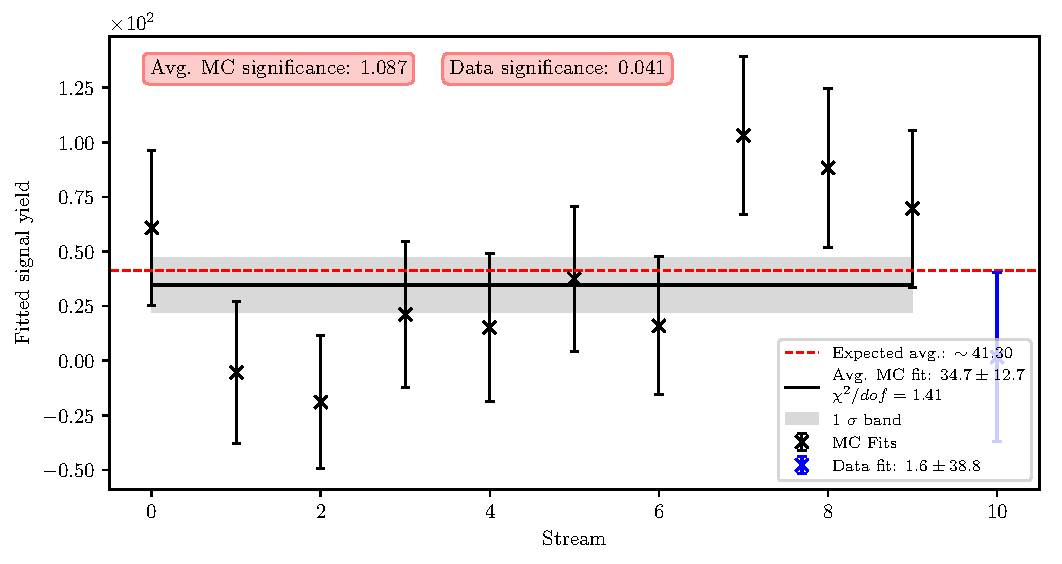
\includegraphics[width=\linewidth]{fig/sig_q2_1}
	\caption{Signal fit result for the $1^{\mathrm{st}}$ $q^2$ window for MC and data in the range $0.000  < q^2 < 1.500$.}
\end{figure}

\begin{figure}[H]
	\centering
	\captionsetup{width=0.8\linewidth}
	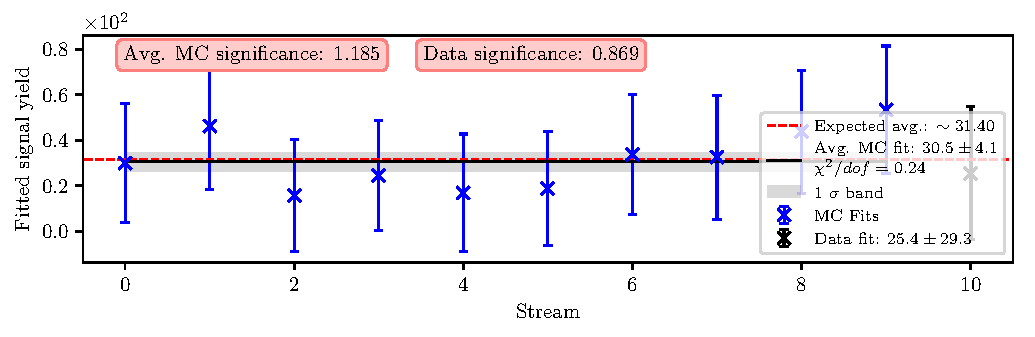
\includegraphics[width=\linewidth]{fig/sig_q2_2}
	\caption{Signal fit result for the $2^{\mathrm{nd}}$ $q^2$ window for MC and data in the range $1.500  < q^2 < 3.000$.}
\end{figure}

\begin{figure}[H]
	\centering
	\captionsetup{width=0.8\linewidth}
	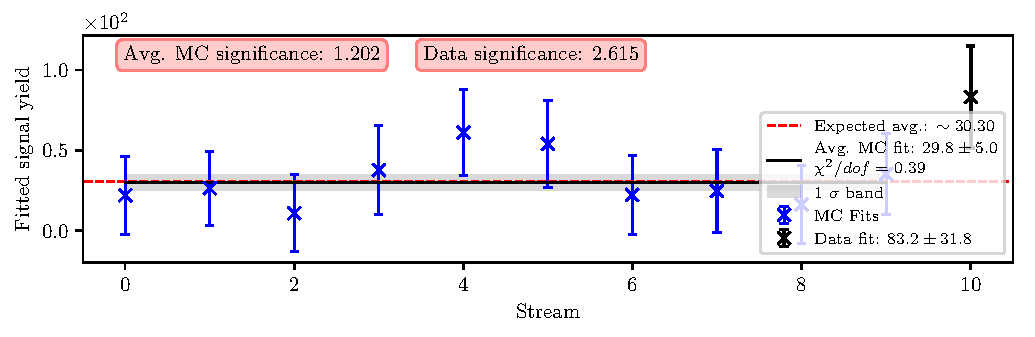
\includegraphics[width=\linewidth]{fig/sig_q2_3}
	\caption{Signal fit result for the $3^{\mathrm{rd}}$ $q^2$ window for MC and data in the range $3.000  < q^2 < 4.500$.}
\end{figure}

\begin{figure}[H]
	\centering
	\captionsetup{width=0.8\linewidth}
	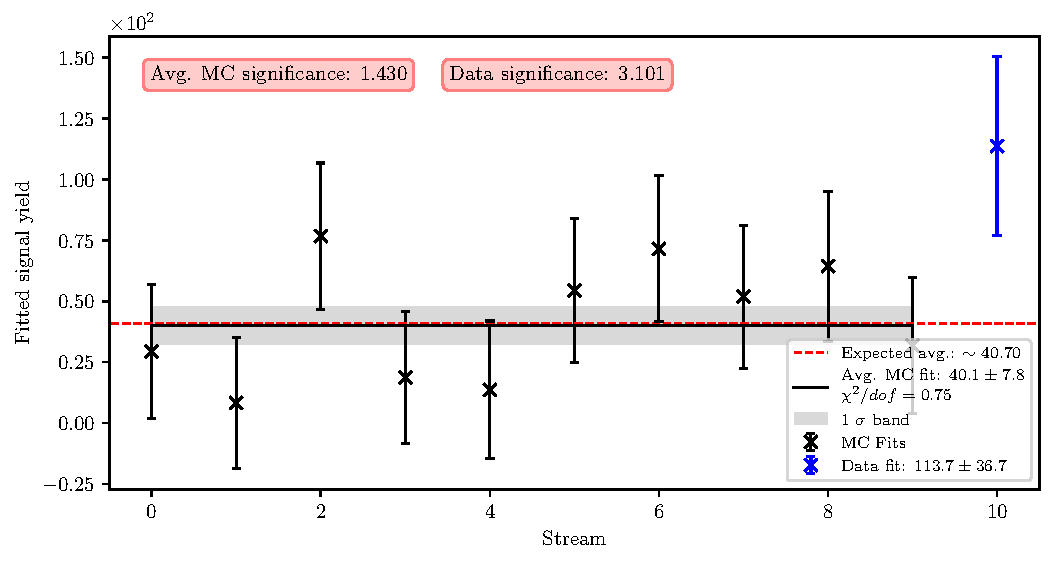
\includegraphics[width=\linewidth]{fig/sig_q2_4}
	\caption{Signal fit result for the $4^{\mathrm{th}}$ $q^2$ window for MC and data in the range $4.500  < q^2 < 6.000$.}
\end{figure}

\begin{figure}[H]
	\centering
	\captionsetup{width=0.8\linewidth}
	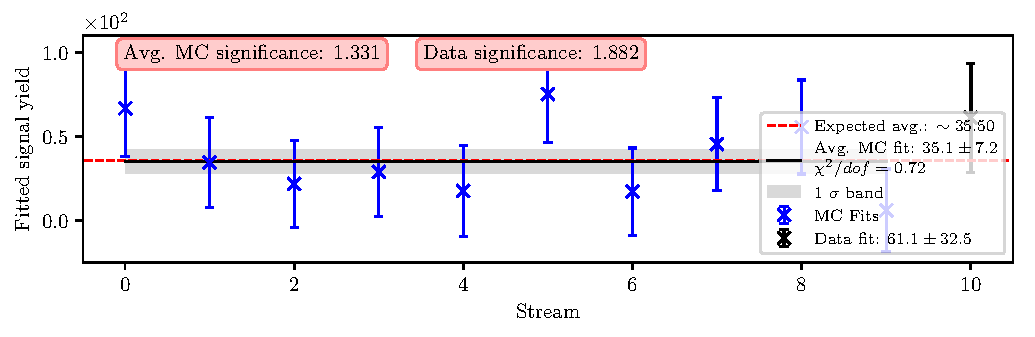
\includegraphics[width=\linewidth]{fig/sig_q2_5}
	\caption{Signal fit result for the $5^{\mathrm{th}}$ $q^2$ window for MC and data in the range $6.000  < q^2 < 7.500$.}
\end{figure}

\begin{figure}[H]
	\centering
	\captionsetup{width=0.8\linewidth}
	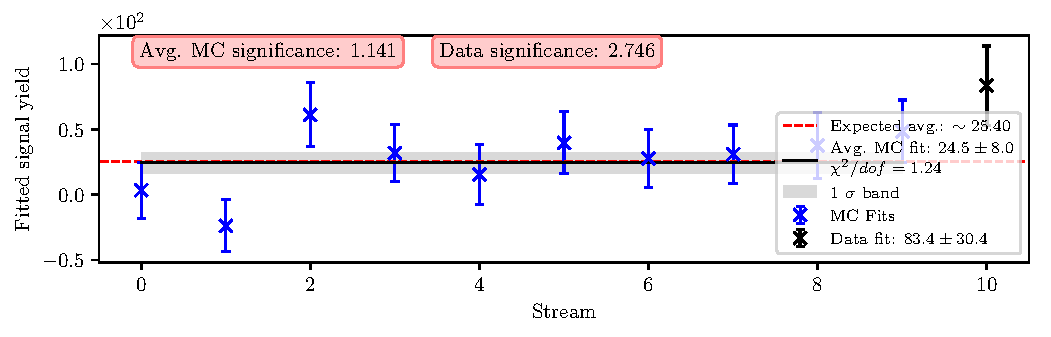
\includegraphics[width=\linewidth]{fig/sig_q2_6}
	\caption{Signal fit result for the $6^{\mathrm{th}}$ $q^2$ window for MC and data in the range $7.500  < q^2 < 9.000$.}
\end{figure}

\begin{figure}[H]
	\centering
	\captionsetup{width=0.8\linewidth}
	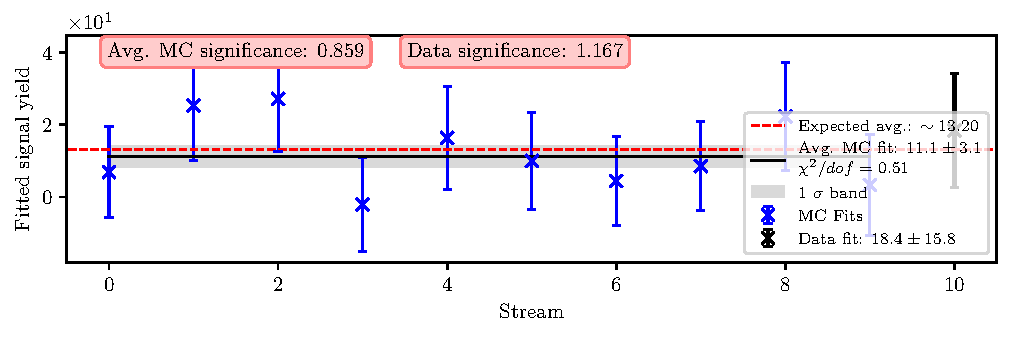
\includegraphics[width=\linewidth]{fig/sig_q2_7}
	\caption{Signal fit result for the $7^{\mathrm{th}}$ $q^2$ window for MC and data in the range $9.000  < q^2 < 10.500$.}
\end{figure}

\begin{figure}[H]
	\centering
	\captionsetup{width=0.8\linewidth}
	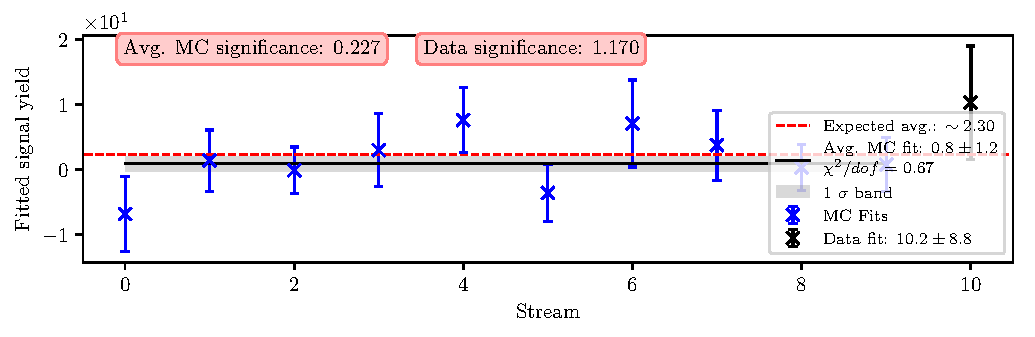
\includegraphics[width=\linewidth]{fig/sig_q2_8}
	\caption{Signal fit result for the $8^{\mathrm{th}}$ $q^2$ window for MC and data in the range $10.500  < q^2 < 12.000$.}
\end{figure}

\begin{figure}[H]
	\centering
	\captionsetup{width=0.8\linewidth}
	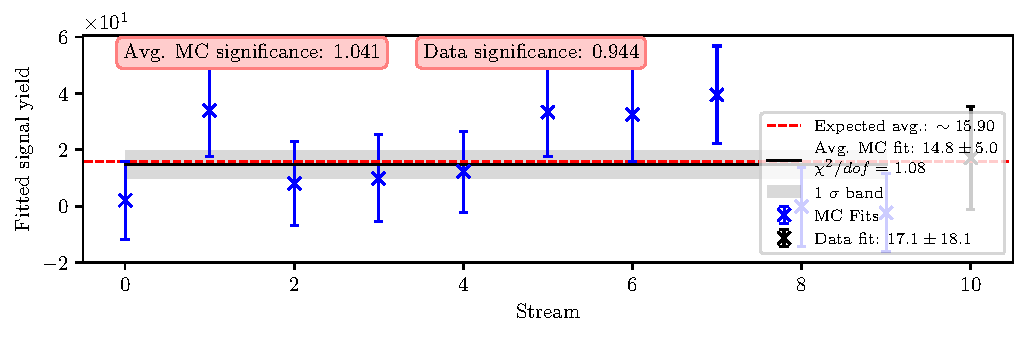
\includegraphics[width=\linewidth]{fig/sig_q2_9}
	\caption{Signal fit result for the $9^{\mathrm{th}}$ $q^2$ window for MC and data in the range $12.000  < q^2 < 13.500$.}
\end{figure}

\begin{figure}[H]
	\centering
	\captionsetup{width=0.8\linewidth}
	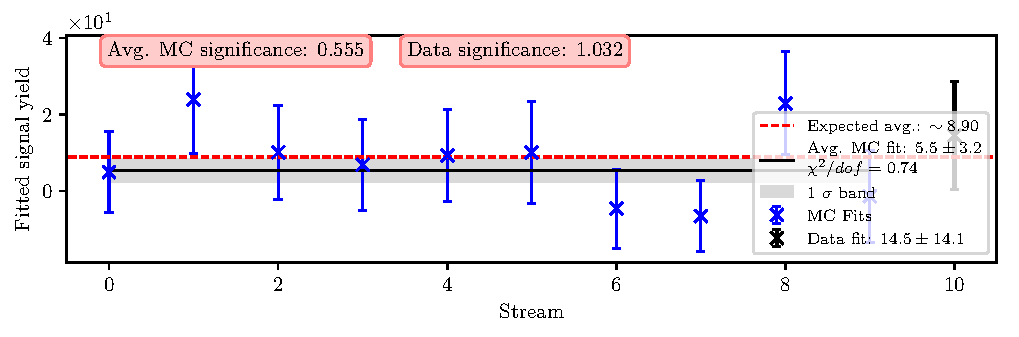
\includegraphics[width=\linewidth]{fig/sig_q2_10}
	\caption{Signal fit result for the $10^{\mathrm{th}}$ $q^2$ window for MC and data in the range $13.500  < q^2 < 15.000$.}
\end{figure}

\begin{figure}[H]
	\centering
	\captionsetup{width=0.8\linewidth}
	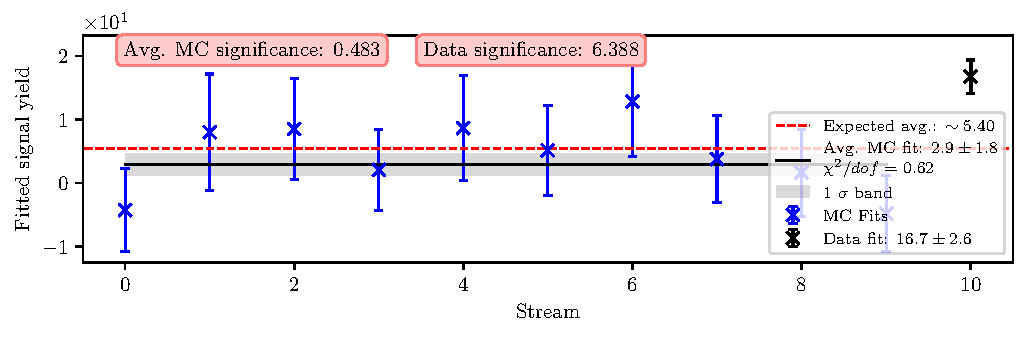
\includegraphics[width=\linewidth]{fig/sig_q2_11}
	\caption{Signal fit result for the $11^{\mathrm{th}}$ $q^2$ window for MC and data in the range $15.000  < q^2 < 16.500$.}
\end{figure}

\begin{figure}[H]
	\centering
	\captionsetup{width=0.8\linewidth}
	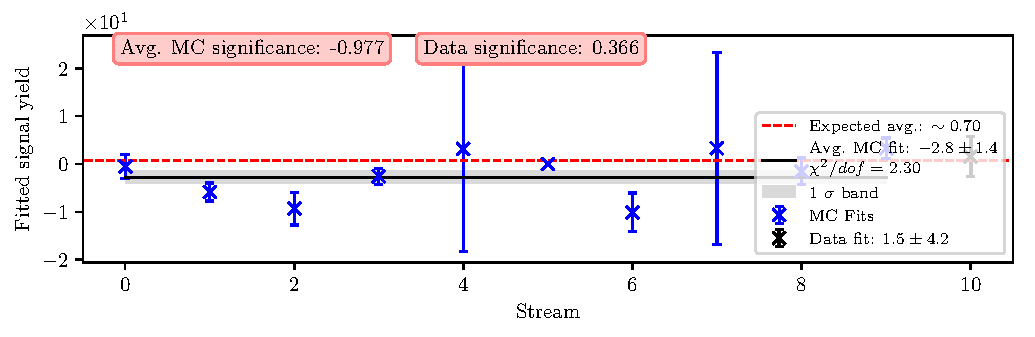
\includegraphics[width=\linewidth]{fig/sig_q2_12}
	\caption{Signal fit result for the $12^{\mathrm{th}}$ $q^2$ window for MC and data in the range $16.500  < q^2 < 18.000$.}
\end{figure}